\chapter{Deployment}
\label{ch:deployment}
\markboth{Deployment}{Deployment}

The deployment subsystem covers only the entry--descent--deployment--inflation (EDDI) slice: from the entry interface at $\approx 200\,\mathrm{km}$ to a confirmed free-float aerobot state at $\approx 55\,\mathrm{km}$. Long-duration float, altitude control, leakage management, and cruise aerodynamics are therefore interfaces to ISRU/Buoyancy, Navigation, Structures, and CDHS rather than deployment-owned design problems.

The chapter provides the following: driving inputs, option enumeration, trade method, selected architecture, first-order performance characteristics, interfaces, compliance, and residual risks. Architecture tags are defined in Table~\ref{tab:architecture-tag-definitions}; reliability is treated in Section~\ref{sec:deployment-pra}.

\subsection*{Design philosophy}
\label{sec:7-1-1}

Technology maturity is judged using the ECSS/ISO TRL framework, where maturity is assessed relative to the intended product and operating environment~\cite{ECSS_E_HB_11A_2017}. Concepts that are clearly below a Venus-relevant qualification path are therefore not listed one by one in this section: too many branches of the design option tree can be rejected on that basis alone, and repeating that argument would not improve the trade.

The resulting design philosophy is conservative: maximise deployment reliability and avoid spending reliability margin on novelty inside the EDDI chain. Reliability is a key driver because deployment is one-shot; if it fails, the mission is lost before the balloon can perform the science. Since the mission's distinctive value lies in the long-duration Venus aerobot rather than in an exotic entry or deployment system, the deployment architecture should use the most mature, separable, and verifiable solution that can deliver the balloon safely to float.

\section{Deployment scope and driving inputs}
\label{sec:dep-reqs}

\subsection{Entry environment}
\label{sec:7-2-1}

The entry masses used here come from the Baseline Report ROM, but they must be corrected for the selected stored-N$_2$ architecture. In the Baseline Report, the N$_2$ gas was included in the operational float mass but not in the launched entry mass, because that architecture assumed the gas would be generated in situ. For the selected stored-N$_2$ option, this is no longer true: the nitrogen is carried into Venus, so it has to be added back into the entry mass before trajectory, TPS, and parachute sizing are checked.

The entry interface and entry speed are taken from Venus-entry heritage missions. For first-order EDDI sizing, the entry interface is set at $\approx 200\,\mathrm{km}$ and the planet-relative entry speed is taken as $\approx 11\,\mathrm{km\,s^{-1}}$.

\begin{table}[H]
\centering
\caption{Deployment-driving entry-environment inputs.}
\label{tab:entry-env}
\small
\renewcommand{\arraystretch}{1.12}
\begin{tabularx}{\textwidth}{@{}p{0.2\textwidth} p{0.2\textwidth} X@{}}
\toprule
\textbf{Input} & \textbf{Value / basis} & \textbf{Deployment use} \\
\midrule
Entry interface & $\approx 200\,\mathrm{km}$ & Start of the entry--descent--deployment--inflation sequence. \\
Entry speed & $\approx 11\,\mathrm{km\,s^{-1}}$ & Initial condition for aeroshell, TPS, and parachute sizing. \\
Baseline ROM entry masses & 93 / 162 / 393\,kg & Baseline Report entry cases before stored-N$_2$ correction. \\
Stored N$_2$ mass & 107 / 180 / 310\,kg & Baseline Report float-mass cases; the 310\,kg case is also supported by the current 55\,km balloon sizing result of 309.61\,kg. \\
Entry hardware fraction & 0.30 / 0.35 / 0.55 & Baseline Report ROM fraction for aeroshell, parachute, separation, and deployment hardware. \\
Deployment trigger & Mach/$q$ window & Sets the parachute extraction and main-canopy deployment box, following planetary parachute practice where deployment conditions are defined by Mach number and dynamic pressure~\cite{CruzLingard2006}. \\
\bottomrule
\end{tabularx}
\end{table}

\begin{table}[htbp]
\centering
\caption{Baseline-to-stored-N$_2$ entry-mass correction.}
\label{tab:dry-wet-entry-correction}
\scriptsize
\setlength{\tabcolsep}{3pt}
\renewcommand{\arraystretch}{1.15}
\begin{tabularx}{\textwidth}{@{}l
>{\centering\arraybackslash}X
>{\centering\arraybackslash}X
>{\centering\arraybackslash}X
>{\centering\arraybackslash}X
>{\centering\arraybackslash}X
>{\centering\arraybackslash}X@{}}
\toprule
\textbf{Case} &
\makecell{\textbf{Baseline}\\\textbf{entry}\\{[kg]}} &
\makecell{\textbf{Float}\\\textbf{hardware}\\{[kg]}} &
\makecell{\textbf{N$_2$}\\\textbf{gas}\\{[kg]}} &
\makecell{\textbf{Min.}\\\textbf{wet}\\{[kg]}} &
\makecell{\textbf{Entry hw.}\\\textbf{frac.}\\{[-]}} &
\makecell{\textbf{Re-est.}\\\textbf{wet}\\{[kg]}} \\
\midrule
Lower    & 93  & 65  & 107 & 200 & 0.30 & 246  \\
Nominal  & 162 & 105 & 180 & 342 & 0.35 & 438  \\
Bounding & 393 & 177 & 310 & 703 & 0.55 & 1082 \\
\midrule
\multicolumn{7}{@{}p{\textwidth}@{}}{\footnotesize
Minimum wet mass:
$m_{\mathrm{wet,min}} = m_{\mathrm{base}} + m_{\mathrm{N_2}}$.
Re-estimated wet mass:
$m_{\mathrm{wet,re\text{-}est}} =
\dfrac{m_{\mathrm{float}} + m_{\mathrm{N_2}}}{1-f_{\mathrm{entry}}}$,
where $f_{\mathrm{entry}}$ is the Baseline Report ROM fraction assigned to aeroshell, parachute, separation, and deployment hardware.
} \\
\bottomrule
\end{tabularx}
\end{table}

The minimum wet mass only adds the stored N$_2$ to the old Baseline entry mass. The re-estimated wet mass is more conservative because the entry hardware is also scaled around the heavier stored-N$_2$ stack. The bounding case is therefore not closed: it shows that carrying all nitrogen at entry can push the deployment system beyond the original 700\,kg mass cap unless the architecture is resized or descoped.

\subsection{Deployment requirements and active assumptions}
\label{sec:dep-active-assumptions}

The Baseline Report defines the deployment requirements, but leaves several values as TBDs or subsystem interfaces. This section only closes the values needed for the architecture trade. These are screening assumptions, not final trajectory, reliability, or qualification results. The mission-level aerobot survival requirement remains $R>0.90$; deployment reliability is therefore treated as a one-shot design driver to be maximised, not as a separately allocated subsystem requirement at Phase~0.

\begin{table}[H]
\centering
\caption{Baseline deployment requirements and chapter-level assumptions used for the architecture trade.}
\label{tab:deployment-retained-reqs}
\footnotesize
\renewcommand{\arraystretch}{1.12}
\begin{tabularx}{\textwidth}{@{}p{0.15\textwidth} X X@{}}
\toprule
\textbf{Baseline input} & \textbf{Baseline requirement / interface} & \textbf{Closure used in this chapter} \\
\midrule
REQ-F-DEP-01, REQ-C-DEP-02 & Deployment must be compatible with the relay-orbiter geometry and reach the operational float altitude. & Hand-off is set to $\approx55\,\mathrm{km}$, near the lower float band, to limit the initial stored-N$_2$ requirement. \\
REQ-F-DEP-03, REQ-F-DEP-12 & Envelope and gondola must deploy without tearing, snagging, entanglement, or post-inflation damage. & Used as the sequence and clearance driver; recontact, tendon entanglement, and gondola-release risks are penalised. \\
REQ-C-DEP-06, REQ-C-SUB-03 & Stored gas must not be released before the required altitude, and the inflation system must remain within its mass allocation. & Stored N$_2$ is included in the wet entry case; premature release, tankage, and inflation mass remain residual risks. \\
REQ-C-DEP-07, REQ-F-DEP-08, REQ-F-DEP-10 & The EDDI chain must survive entry loads, remain dynamically stable, and decelerate to a deployable state. & A $200\,g_0$ load cap and Mach/$q$ parachute trigger box are used as first-order screening limits, based on Venus ballistic-entry studies using $200\,g$ as a science-payload mechanical limit~\cite{Prabhu2013VenusEntry}. \\
REQ-F-DEP-09, REQ-C-SUB-04 & The stack must fit the entry capsule, while aeroshell and parachute mass remain within the Baseline allocation. & Used as the main packaging and EDL-mass closure. \\
REQ-F-DEP-11, REQ-F-DEP-13--15 & Heat-shield orientation, jettison, structural survival, and thermal survival must close during Venus entry. & Treated as aeroshell and separation constraints; avoidable jettison or recontact risks are penalised. \\
REQ-F-DEP-04 & Successful deployment must be confirmed after release and inflation. & Requires CDHS-coupled deployment-status confirmation after free-float hand-off. \\
REQ-C-MIS-02, REQ-C-MIS-03 & Total aerobot mass is limited to $700\,\mathrm{kg}$ and each aerobot must exceed $90\%$ mission survival probability. & Applies the dry/wet mass correction; deployment reliability is maximised, but no fixed subsystem allocation is claimed. \\
REQ-F-LAU-04--06 & Deployment must not activate before Venus entry, launch locks must release after arrival, and interfaces must be verified before launch. & Folded into release logic and AIT rather than traded as separate architecture drivers. \\
\bottomrule
\end{tabularx}
\end{table}

Altitude control, envelope sizing, leakage management, cruise aerodynamics, and long-duration material ageing remain subsystem interfaces unless they affect initial fill, separation, or free-float hand-off.

\clearpage

\begin{landscape}
\thispagestyle{plain}

\section{Design option tree}
\label{sec:7-3}

The DOT in Figure~\ref{fig:DOTD} defines the deployment-side option space. The selection argument is made in Section~\ref{sec:dep-integration}, where low-maturity and weak-reliability combinations are removed.

\vspace{0.5em}

\begin{figure}[H]
    \centering
    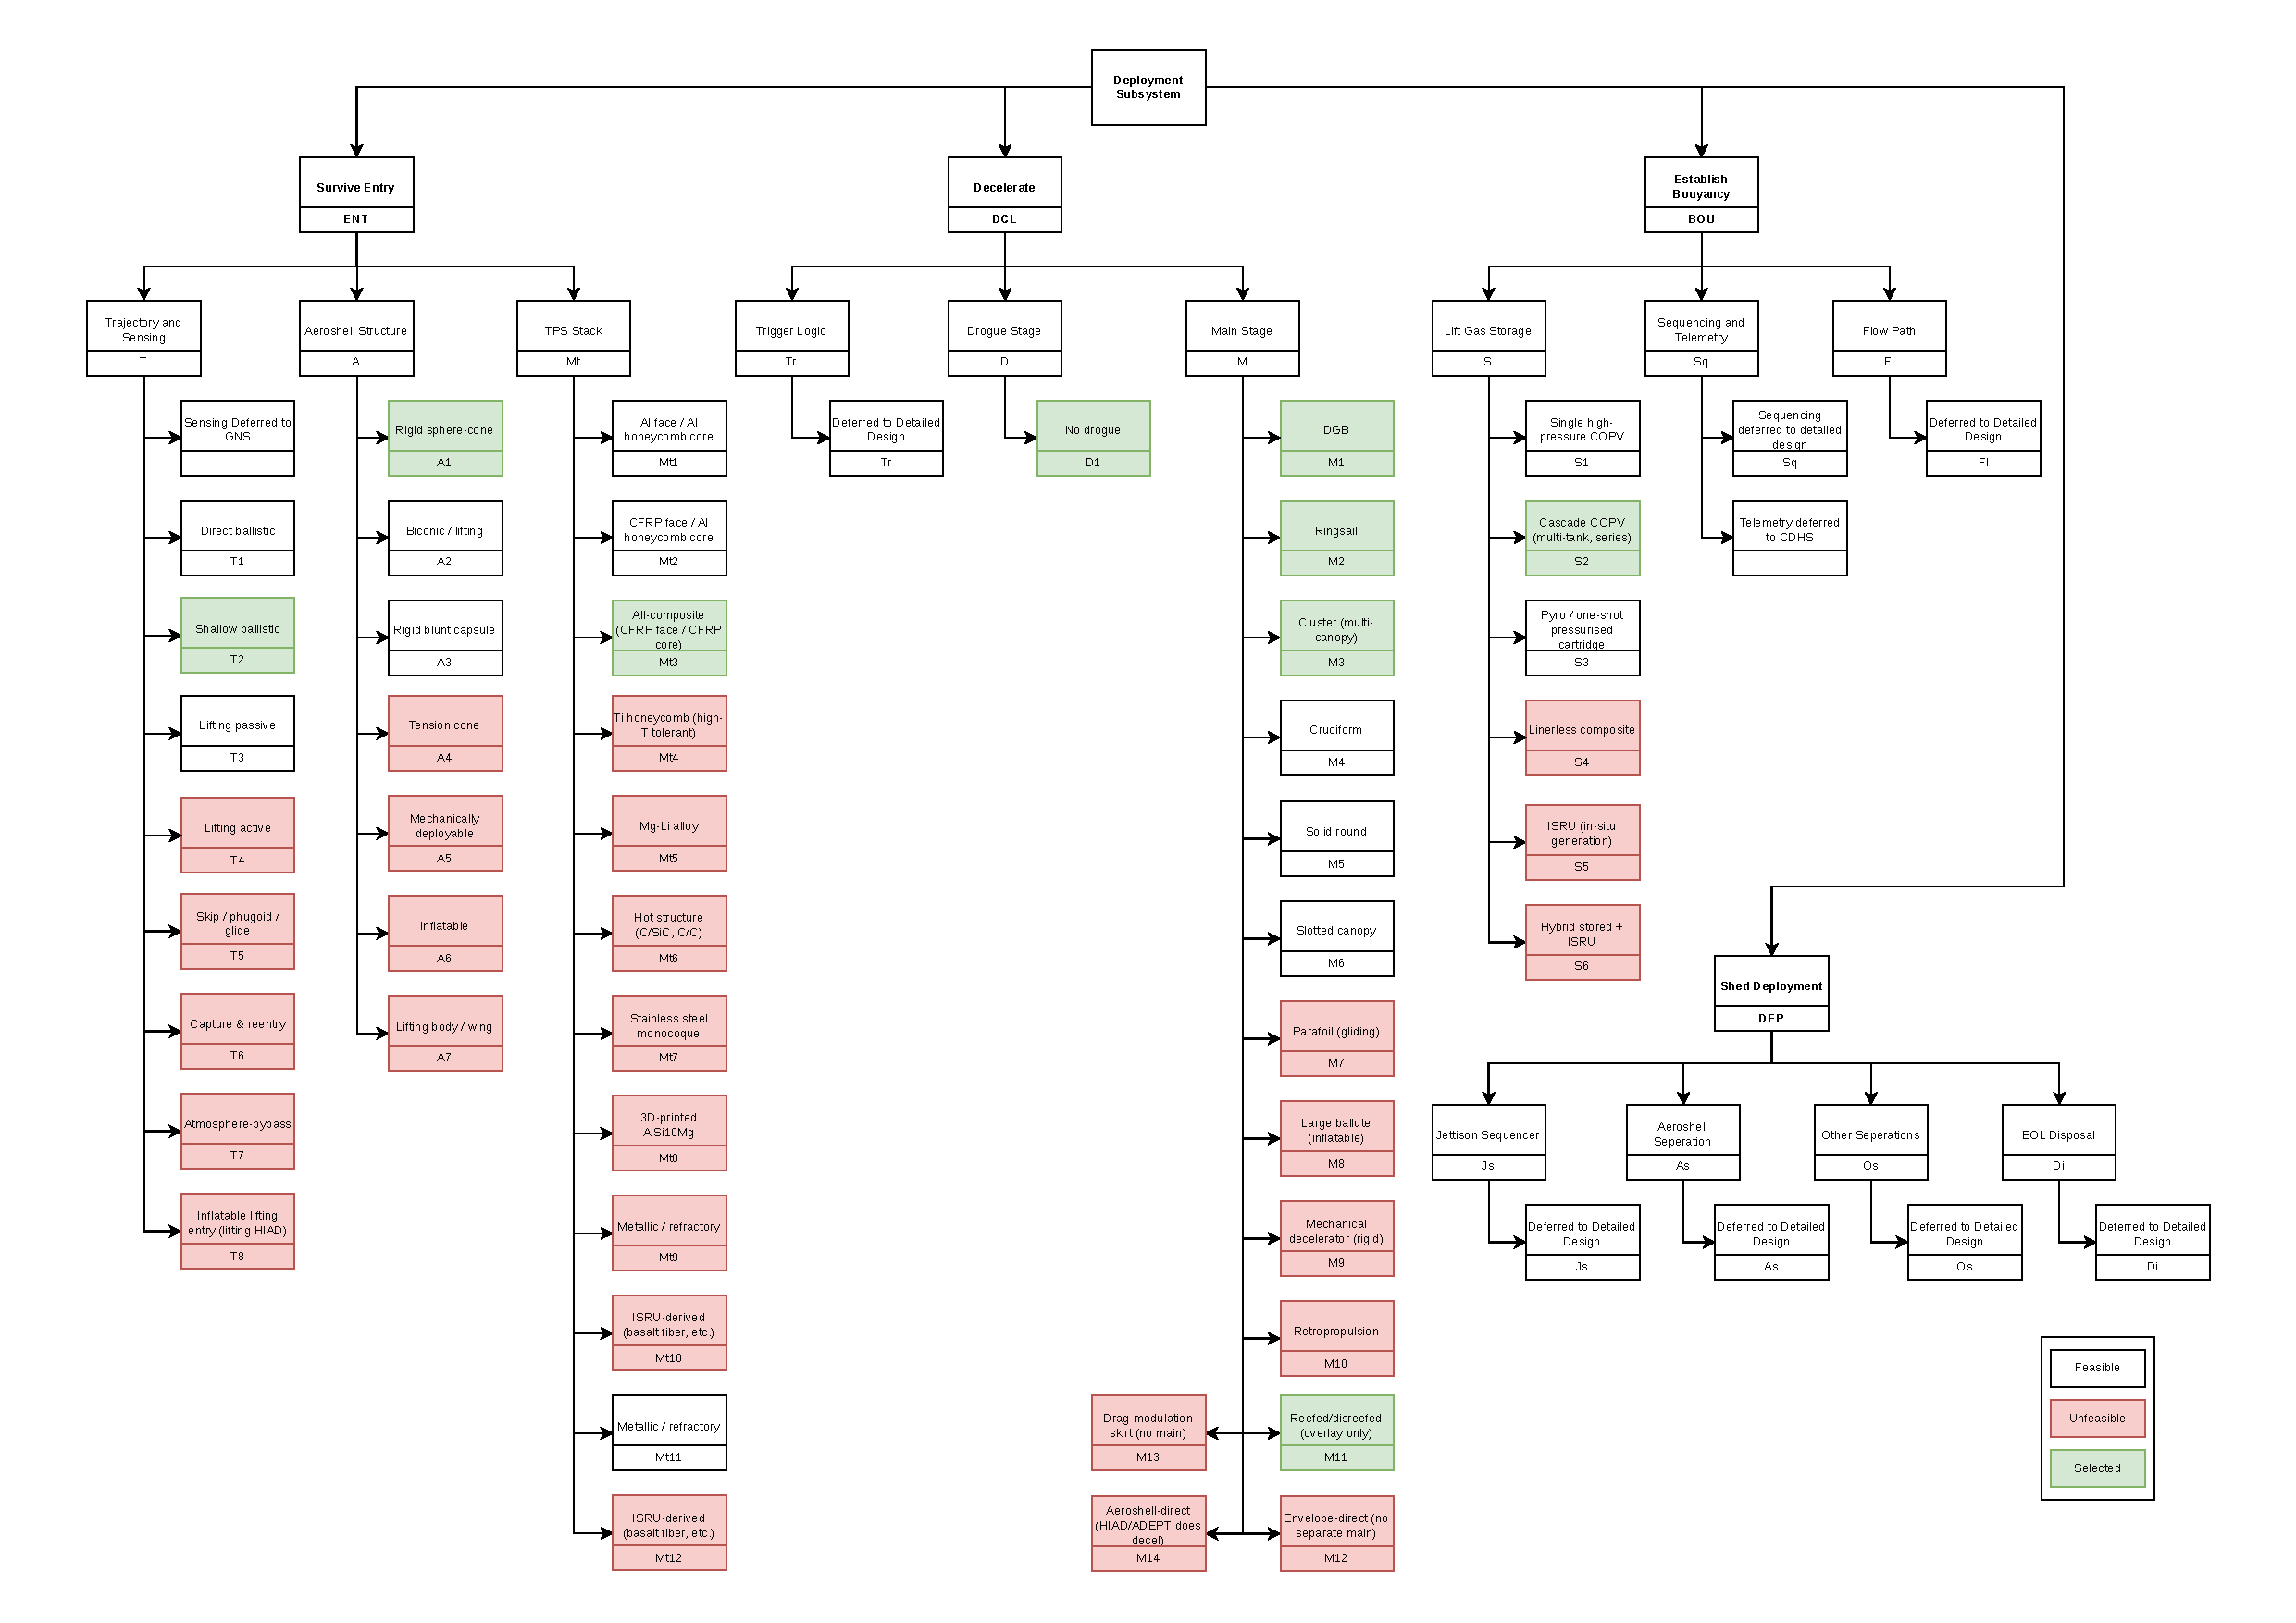
\includegraphics[
        width=\linewidth,
        height=0.8\textheight,
        keepaspectratio
    ]{fig/DOT_Dep.pdf}
    \caption{Design Option Tree for the deployment subsystem.}
    \label{fig:DOTD}
\end{figure}

\end{landscape}

\clearpage


\section{Trade method and architecture selection}
\label{sec:dep-method}

The trade is split into two tracks. Track~1 selects the best independent DOT options, giving the audit tuple $(T^{*},A^{*},M_t^{*},S^{*},M^{*})=(T2,A1,Mt3,S2,M2)$. Track~2 then reopens the architecture space and selects the most reliable feasible deployment architecture. The material axis $M_t$ is not included in the main Cartesian search because material choice is resolved in a parallel trade. Technology maturity is used as a hard filter: Only architectures with TRL~$\geq 7$ today and a credible path to TRL~9 by PDR are retained. This keeps deployment low-risk, reserving the technology risk budget for the novel balloon and long-duration float system. This keeps the lower-maturity risk budget on the floating subsystem rather than the one-shot EDDI chain.

The resulting cascade is summarised in Table~\ref{tab:track2-filter-cascade}. The final selection is $\varepsilon_{\mathrm{RX}}$--Mt3, which maximises reliability while remaining within the entry-mass cap.

\begin{table}[H]
\centering
\footnotesize
\caption{Deployment architecture down-selection cascade.}
\label{tab:track2-filter-cascade}
\renewcommand{\arraystretch}{1}
\setlength{\tabcolsep}{6pt}

\begin{tabularx}{\textwidth}{
@{}
>{\raggedright\arraybackslash}p{0.28\textwidth}
>{\centering\arraybackslash}p{0.08\textwidth}
X
@{}
}
\toprule
\textbf{Stage} & \textbf{Cases} & \textbf{Outcome} \\
\midrule

Raw DOT space
& 4032
& Full $(T,A,S,M)$ architecture space; $M_t$ handled separately. \\

Compatibility filters
& $\approx 120$
& Physically or interface-incoherent combinations removed. \\

TRL filter
& 26
& Only architectures with TRL~$\geq 7$ today and credible path to TRL~9 retained. \\

Class-champion sweep
& 5
& Only $\alpha$, $\varepsilon$, $M_t$, and $T$ families retain feasible contenders. \\

Final selection
& 1
& $\varepsilon_{\mathrm{RX}}$--Mt3 selected: $R=0.992$ with 95\,\% CI $[0.985,0.996]$, $500\,\mathrm{kg}$ ROM entry mass, within the $700\,\mathrm{kg}$ cap. \\

\bottomrule
\end{tabularx}
\end{table}

\subsection{Track 1: independent solution}
\label{sec:track1-independent}
\label{sec:7-3-1}
\label{sec:7-3-3}
\label{sec:dep-d12b}
\label{sec:7-3-2}
\label{sec:dep-d44}
\label{sec:dep-d31}

Each deployment axis is first scored on its own. Detailed archived-branch explanations are removed from the MTR chapter; the key selection logic is retained in Table~\ref{tab:track1-setup}.

\begin{table}[ht]
\centering
\renewcommand{\arraystretch}{1}
\small
\caption{Selected Track~1 independent deployment setup.}
\label{tab:track1-setup}
\label{tab:lift-payoff-screen}
\label{tab:d11-trajectory-screening}
\label{tab:d13-structure-screening}
\label{tab:d12-material-screening}
\label{tab:main-deploy-trigger}
\label{tab:d23-descent-screening}
\label{tab:d31-storage-screening}
\setlength{\tabcolsep}{5pt}
\begin{tabularx}{\textwidth}{@{}p{0.18\textwidth} p{0.18\textwidth} p{0.18\textwidth} X@{}}
\toprule
\textbf{Axis} & \textbf{Selected option} & \textbf{Fallback} & \textbf{Reason} \\
\midrule
Trajectory class & T2 shallow ballistic & T1 steep ballistic & Uses Venus heritage and keeps peak load low without adding lift hardware. \\
Aeroshell architecture & A1 rigid sphere-cone & A3 blunt capsule & Best blunt-body heritage path for a non-lifting trajectory~\cite{Seiff1991,Garvin2022,Steltzner2014}. \\
Aeroshell material & Mt3 all-composite face/core & Mt2 CFRP/Al core & Best mass/interface trade, but coupon qualification remains DEP-2. \\
Lift-gas storage & S2 cascaded COPVs & S3 cartridge & Avoids single-point inflation failure and supports cross-strapped inflation strings. \\
Main descent system & M2 DGB + reefed ringsail cluster & M1 single DGB & Uses DGB heritage with a calmer terminal hand-off~\cite{Knacke1992,CruzLingard2006,Witkowski2013}. \\
\midrule
\multicolumn{4}{@{}l@{}}{\textbf{Track~1 tuple:} $(T^*,A^*,Mt^*,S^*,M^*)=(T2,A1,Mt3,S2,M2)$.} \\
\bottomrule
\end{tabularx}
\end{table}

The main rejected branches are not design drivers. Lifting trajectories add CG-offset, asymmetric TPS, RCS, or GN\&C mass for little benefit because VISTA deploys to a cloud-layer float state rather than a surface landing target. Deployable/inflatable aeroshells and lifting HIAD options remain below the Venus-relevant maturity needed for a one-shot deployment claim~\cite{Mankins1995,Grinspoon2010,Sagdeev1986}. Mt2 stays as the fallback if the Mt3 coupon programme fails.

\subsection{Track 2: integrated architecture ranking}

Track~2 checks whether separate DOT choices can be combined without creating a hidden interface or reliability penalty. The integration vectors are only an internal trade notation.

\begin{table}[H]
    \centering
    \renewcommand{\arraystretch}{1}
    \footnotesize
    \caption{Integration vector taxonomy for the deployment trade space.}
    \label{tab:integration_vectors}
    \begin{tabularx}{\linewidth}{p{0.10\linewidth} p{0.20\linewidth} X p{0.25\linewidth}}
        \toprule
        \textbf{Vector} & \textbf{Axes collapsed} & \textbf{Mechanism} & \textbf{Status} \\
        \midrule
        $\alpha$ & None & Heritage layout; all axes remain separate. & Reference backbone \\
        $\beta$ & A + M & Aeroshell also works as decelerator. & Archived; low TRL \\
        $\gamma$ & S + M & Stored gas inflates a ballute, then feeds envelope. & Archived; reliability too low \\
        $\delta$ & M + envelope & Envelope replaces main decelerator. & Archived; Buoyancy-owned \\
        $\varepsilon$ & S + A & Storage and aeroshell structure share load paths. & Selected in $\varepsilon_{\mathrm{RX}}$-Mt3 \\
        $\zeta$ & A + M + envelope & One inflatable handles entry, deceleration, and float. & Archived; TRL~1 \\
        $\eta$ & T + A & Lifting trajectory needs a lifting aeroshell. & Alternate; reliability too low \\
        $\theta$ & S + M + envelope & One gas reserve supports ballute and envelope. & Archived; CCF dominated \\
        $\iota$ & S + A + M & Storage, aeroshell, and descent tied into one load path. & Archived; insufficient mass/$R$ data \\
        \bottomrule
    \end{tabularx}
\end{table}

\begin{table}[H]
\centering
\small
\renewcommand{\arraystretch}{1}
\caption{Architecture tags used in the deployment ranking.}
\label{tab:architecture-tag-definitions}
\begin{tabularx}{\textwidth}{@{}p{0.22\textwidth} p{0.24\textwidth} X@{}}
\toprule
\textbf{Tag} & \textbf{Role} & \textbf{Definition} \\
\midrule
Track~1 tuple & Independent optimum & $(T2,A1,Mt3,S2,M2)$ selected axis-by-axis without integration credit. \\
$\alpha_1$ & Heritage reference & Single-string uncoupled reference using the T2/A1 backbone, Mt2 fallback material, S1 single COPV, and M1 single DGB. \\
$\alpha_{\mathrm{R3}}$-Mt3 & Redundancy rung & $\alpha_1$ with Mt3 and three-way redundant/cross-strappable P8 inflation strings. \\
$\alpha_{\mathrm{R6}}$-Mt3 & Redundancy rung & Mt3 case with six-way critical-string redundancy; common-cause failure dominates. \\
$\varepsilon_{\mathrm{RX}}$-Mt3 & Selected architecture & T2/A1/Mt3/S2/M2 with $\varepsilon_1$ S+A coupling, functional diversity, and supplier separation. \\
\bottomrule
\end{tabularx}
\end{table}

Figure~\ref{fig:track2_mass_reliability} shows the final ranking. The lightest options were checked, but their reliability is limited by single-string or common-cause failure modes. Among architectures with complete DSE-level mass and reliability estimates, $\varepsilon_{\mathrm{RX}}$-Mt3 gives the highest achievable deployment reliability while remaining within the entry-mass and packaging constraints.

\begin{figure}[H]
\centering
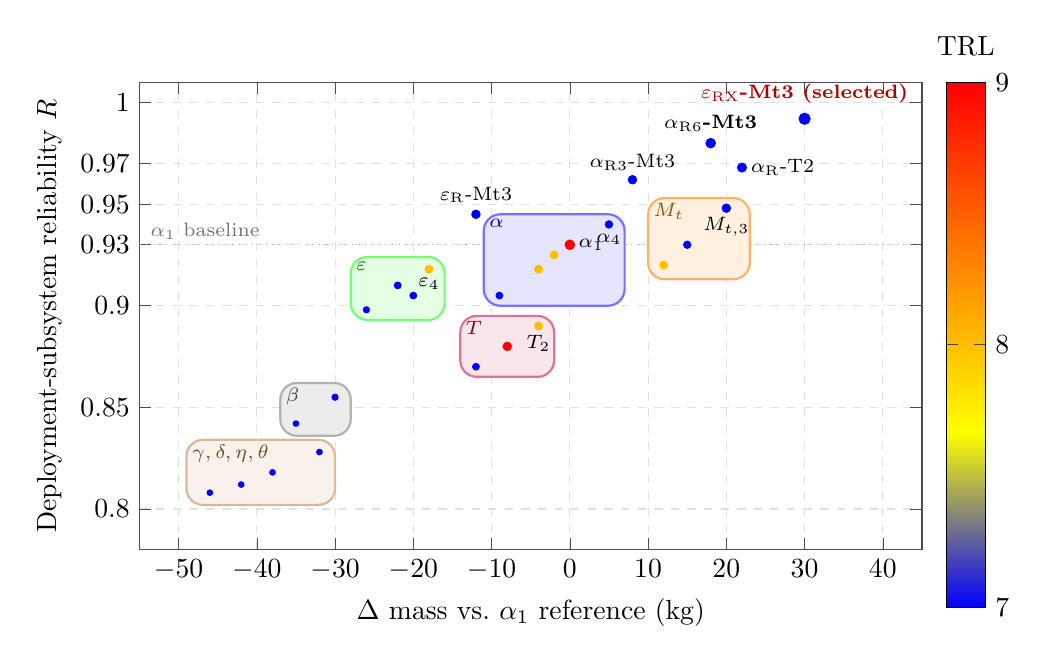
\begin{tikzpicture}[
  label/.style={font=\scriptsize, inner sep=1pt},
  famlabel/.style={font=\scriptsize\itshape, inner sep=1pt},
  keylabel/.style={font=\scriptsize\bfseries, inner sep=1pt},
]
\begin{axis}[
  width=0.95\linewidth,
  height=0.62\linewidth,
  xlabel={$\Delta$ mass vs.\ $\alpha_1$ reference (kg)},
  ylabel={Deployment-subsystem reliability $R$},
  xmin=-55, xmax=45,
  ymin=0.78, ymax=1.01,
  xtick={-50,-40,-30,-20,-10,0,10,20,30,40},
  ytick={0.80,0.85,0.90,0.93,0.95,0.97,1.00},
  yticklabel style={/pgf/number format/.cd, fixed, precision=2},
  grid=major,
  grid style={dashed, black!12},
  axis line style={black!70},
  tick style={black!70},
  enlargelimits=false,
  clip=true,
  scatter/use mapped color={draw=mapped color, fill=mapped color},
  point meta min=7,
  point meta max=9,
  colorbar,
  colorbar style={
    title={TRL},
    ylabel={},
    ytick={7,8,9},
    height=0.55\linewidth,
  },
]
% --- alpha_1 baseline reference line ---
\addplot [draw=black!35, thin, dotted, domain=-55:45] {0.93};

% =========================================================
% FAMILY CLUSTER BACKDROPS (behind markers)
% =========================================================
\draw[fill=blue!10,    draw=blue!55,    thick, rounded corners=6pt]
  (axis cs:-11,0.900) rectangle (axis cs:7,0.945);
\draw[fill=green!10,   draw=green!55,   thick, rounded corners=6pt]
  (axis cs:-28,0.893) rectangle (axis cs:-16,0.924);
\draw[fill=orange!12,  draw=orange!60,  thick, rounded corners=6pt]
  (axis cs:10,0.913) rectangle (axis cs:23,0.953);
\draw[fill=purple!10,  draw=purple!55,  thick, rounded corners=6pt]
  (axis cs:-14,0.865) rectangle (axis cs:-2,0.895);
\draw[fill=gray!15,    draw=gray!60,    thick, rounded corners=6pt]
  (axis cs:-37,0.836) rectangle (axis cs:-28,0.862);
\draw[fill=brown!10,   draw=brown!55,   thick, rounded corners=6pt]
  (axis cs:-49,0.802) rectangle (axis cs:-30,0.834);

% Family tags (compact symbols, INSIDE each box, top-left corner)
\node[famlabel, blue!60!black,   anchor=north west] at (axis cs:-10.7,0.944)  {$\alpha$};
\node[famlabel, green!50!black,  anchor=north west] at (axis cs:-27.7,0.923)  {$\varepsilon$};
\node[famlabel, orange!60!black, anchor=north west] at (axis cs:10.3,0.952)   {$M_t$};
\node[famlabel, purple!60!black, anchor=north west] at (axis cs:-13.7,0.894)  {$T$};
\node[famlabel, gray!50!black,   anchor=north west] at (axis cs:-36.7,0.861)  {$\beta$};
\node[famlabel, brown!60!black,  anchor=north west] at (axis cs:-48.7,0.833)  {$\gamma,\delta,\eta,\theta$};

% =========================================================
% DATA POINTS (26 = 21 single-stack + 5 composites)
% =========================================================
\addplot[
  scatter,
  only marks,
  mark=*,
  scatter src=explicit,
  visualization depends on={\thisrow{size} \as \markersize},
  mark options={scale=\markersize},
]
table[
  x=dm,
  y=R,
  meta=TRL,
  row sep=\\
] {
dm     R      TRL  size\\
% --- alpha family (5) ---
0      0.930  9    0.85\\
-4     0.918  8    0.70\\
-9     0.905  7    0.60\\
5      0.940  7    0.65\\
-2     0.925  8    0.70\\
% --- epsilon family (4) ---
-26    0.898  7    0.55\\
-22    0.910  7    0.60\\
-20    0.905  7    0.60\\
-18    0.918  8    0.70\\
% --- M_t family (3) ---
12     0.920  8    0.70\\
15     0.930  7    0.65\\
20     0.948  7    0.75\\
% --- T family (3) ---
-8     0.880  9    0.75\\
-4     0.890  8    0.70\\
-12    0.870  7    0.60\\
% --- beta family (2) ---
-30    0.855  7    0.55\\
-35    0.842  7    0.50\\
% --- gamma / delta / eta / theta (4 singletons) ---
-32    0.828  7    0.50\\
-38    0.818  7    0.50\\
-42    0.812  7    0.50\\
-46    0.808  7    0.50\\
% --- composites (5; individually labelled) ---
-12    0.945  7    0.75\\
8      0.962  7    0.75\\
18     0.980  7    0.85\\
30     0.992  7    1.00\\
22     0.968  7    0.80\\
};

% =========================================================
% KEY-POINT LABELS (placed to avoid all collisions)
% =========================================================
% Selected architecture
\node[keylabel, anchor=south, red!70!black] at (axis cs:30,0.998)
  {$\varepsilon_{\mathrm{RX}}$-Mt3 (selected)};

% Other composites (stacked above their markers)
\node[keylabel, anchor=south] at (axis cs:18,0.984)
  {$\alpha_{\mathrm{R6}}$-Mt3};
\node[label, anchor=south] at (axis cs:8,0.965)
  {$\alpha_{\mathrm{R3}}$-Mt3};
\node[label, anchor=west] at (axis cs:22.7,0.968)
  {$\alpha_{\mathrm{R}}$-T2};
\node[label, anchor=south] at (axis cs:-12,0.949)
  {$\varepsilon_{\mathrm{R}}$-Mt3};

% alpha_1 ladder anchor (inside alpha-box, just right of marker)
\node[label, anchor=west] at (axis cs:0.7,0.930)  {$\alpha_1$};

% Single-stack family champions (below their markers, inside the boxes,
% so they never collide with composite labels above)
\node[label, anchor=north] at (axis cs:5,0.937)    {$\alpha_4$};
\node[label, anchor=north] at (axis cs:20,0.945)   {$M_{t,3}$};
\node[label, anchor=north] at (axis cs:-4,0.887)   {$T_2$};
\node[label, anchor=north] at (axis cs:-18,0.915)  {$\varepsilon_4$};

% Reference-line label (far-left, in dead space)
\node[label, anchor=south west, black!55] at (axis cs:-54,0.931)
  {$\alpha_1$ baseline};
\end{axis}
\end{tikzpicture}
\caption{Mass payoff versus reliability for the 26 Track~2 architectures surviving the TRL$\geq$7 coherence cut, grouped by family. Six coloured regions enclose the single-stack families that retain at least one entrant after the class-champion sweep ($\alpha$, $\varepsilon$, $M_t$, $T$, $\beta$, and the low-weight singleton families $\gamma,\delta,\eta,\theta$); the five composite architectures sit outside the boxes and are labelled individually. Horizontal axis is $\Delta m$ relative to the $\alpha_1$ heritage reference; vertical axis is deployment-subsystem reliability $R$; marker colour encodes TRL and marker size is proportional to family weight after the sweep. $\varepsilon_{\mathrm{RX}}$-Mt3 is the selected architecture.}
\label{fig:track2_mass_reliability}
\end{figure}

\subsection{Reliability methodology (Probabilistic Risk Assessment)}
\label{sec:deployment-pra}
\label{sec:dep-pra}

A short PRA is used because deployment is one-shot: if inflation fails, the mission is lost. The direct Venus balloon precedent is limited to the two Vega balloons, so the inflation claim cannot be made from Venus flight count alone~\cite{Sagdeev1986,Linkin1986}. TPS and parachute functions have stronger Venus, Mars, and Earth heritage and are kept as series factors~\cite{Seiff1991,Garvin2022,Steltzner2014,Witkowski2013}.

\begin{table}[H]
    \centering
    \footnotesize
    \renewcommand{\arraystretch}{1}
    \caption{Deployment phase reliability budget for $\varepsilon_{\mathrm{RX}}$-Mt3.}
    \label{tab:deployment_phase_reliability}
    \begin{tabularx}{\linewidth}{p{0.08\linewidth} X X p{0.13\linewidth}}
        \toprule
        \textbf{Phase} & \textbf{Event} & \textbf{Dominant failure mode} & \textbf{$R_i$} \\
        \midrule
        P1 & Cruise-stowage release & Launch-lock fail-to-retract & 0.9995 \\
        P2 & Entry-interface acquisition & Attitude excursion / spin loss & 0.9990 \\
        P3 & Hypersonic deceleration & Mt3 face/core bond-line failure & 0.9995 \\
        P4 & Mach-trigger sense & Sensor or sequencer fault & 0.9995 \\
        P5 & Main mortar + DGB extract & Mortar misfire / line tangle & 0.9995 \\
        P6 & Reefed ringsail descent & Reefing-cutter failure & 0.9995 \\
        P7 & Forebody / backshell jettison & Recontact or NSI misfire & 0.9995 \\
        P8 & Envelope inflation & Regulator / manifold failure & 0.9970 \\
        P9 & Parachute release / float capture & Release-pyro misfire / pendular runaway & 0.9990 \\
        \bottomrule
    \end{tabularx}
\end{table}

\begin{equation}
    R_{\mathrm{deploy}}=\prod_{i=1}^{9}R_i=0.992 .
    \label{eq:deployment_series_reliability}
\end{equation}

P8 contributes the largest single loss term, so the inflation system is modelled as a set of redundant inflation strings with a common-cause $\beta$-factor~\cite{Mosleh1998}:
\begin{equation}
    Q_{\mathrm{set}} =
    (1-\beta)
    \sum_{k=k_{\min}}^{M}
    \binom{M}{k} q^k (1-q)^{M-k}
    + \beta q .
    \label{eq:beta_factor_model}
\end{equation}
The selected case uses $\beta=0.005$ only as a conditional screening value: it requires supplier separation and functional diversity between inflation strings. Since the two Vega balloon flights alone are too small a data set to justify this value, P8 is treated as an augmented reference-class estimate rather than a flight-count-derived probability:
\begin{equation}
    R \mid \mathrm{data}
    \sim
    \mathrm{Beta}\!\left(\alpha_0+s,\beta_0+n-s\right),
    \label{eq:bayesian_reliability_update}
\end{equation}

Here, $s$ successful deployments in $n$ comparable trials update the prior reliability distribution; with only two Vega balloon flights, the result remains prior-dominated.

\begin{table}[H]
\centering
\footnotesize
\renewcommand{\arraystretch}{1}
\caption{Condensed reliability ladder and common-cause sensitivity.}
\label{tab:reliability_ladder}
\begin{tabularx}{\textwidth}{@{}p{0.22\textwidth} p{0.12\textwidth} p{0.14\textwidth} X@{}}
\toprule
\textbf{Case} & \textbf{$\Delta m$} & \textbf{$R_{\mathrm{deploy}}$} & \textbf{Meaning} \\
\midrule
$\alpha_1$ & 0\,kg & 0.930 & Single-string heritage reference. \\
$\alpha_{\mathrm{R3}}$-Mt3 & $-5$\,kg & 0.960 & Three-way inflation redundancy; Mt3 mass saving still offsets added string hardware. \\
$\alpha_{\mathrm{R6}}$-Mt3 & $+15$\,kg & 0.980 & Six-way redundancy; further gains are already common-cause limited. \\
$\varepsilon_{\mathrm{RX}}$-Mt3, $\beta=0.005$ & $+30$\,kg & 0.992 & Selected screening case, conditional on supplier separation and functional diversity. \\
$\varepsilon_{\mathrm{RX}}$-Mt3, $\beta=0.020$ & $+30$\,kg & 0.987 & Sensitivity case if redundant strings collapse to common components or common procurement. \\
\bottomrule
\end{tabularx}

\vspace{0.25em}
\begin{minipage}{0.96\textwidth}
\footnotesize
\emph{Note.} $\Delta m$ is measured relative to the $\alpha_1$ entry-mass reference and includes only Track~2 architecture-level deltas: Mt3 material saving, added inflation-string hardware, isolation hardware, and S+A coupling provisions. It is not a full subsystem mass re-roll-up.
\end{minipage}
\end{table}

The headline screening value is therefore $R_{\mathrm{deploy}}=0.992$, conditional on the P8 prior, the unresolved S2 string-success model, and the low common-cause assumption. The $\beta=0.020$ case shows that the selected architecture only retains its reliability advantage if procurement and functional diversity are preserved.

\subsection{Selected architecture: \texorpdfstring{$\varepsilon_{\mathrm{RX}}$}{epsilonRX}-Mt3}
\label{sec:8-4}

The selected architecture is $\varepsilon_{\mathrm{RX}}$-Mt3: T2 shallow-ballistic entry, A1 rigid sphere-cone aeroshell, Mt3 all-composite face/core material, S2 cascaded COPV storage, M2 DGB-pilot plus reefed-ringsail descent, and $\varepsilon_1$ S+A coupling. The $\varepsilon_1$ coupling routes the cascaded COPVs along gondola/aeroshell load paths. During EDDI they store staged inflation gas; after P9 they are retained as a candidate structural load path, pending Structures verification of end-fitting loads, pressure-vessel external-load allowables, mounting saddles, and knockdown factors.

\paragraph*{System sizing.} The selected architecture is carried forward with a ROM entry mass of $m_\text{entry}\approx500\,\mathrm{kg}$, about $+30\,\mathrm{kg}$ relative to the $\alpha_1$ heritage reference. The retained float mass is $m_\text{float}\approx120\,\mathrm{kg}$, so roughly $345\,\mathrm{kg}$ is shed by float capture: $\approx155\,\mathrm{kg}$ aeroshell/TPS and $\approx190\,\mathrm{kg}$ deployment and delivery hardware. The forebody is a $45^\circ$ sphere-cone with drag area $S_\text{ref}\approx12\,\mathrm{m^2}$ and ballistic coefficient $\beta^{*}\approx90\,\mathrm{kg/m^2}$. The entry-load screen uses a $200\,g_0$ cap, consistent with Venus ballistic-entry studies that use $200\,g$ as a payload mechanical limit~\cite{Prabhu2013VenusEntry}.

\paragraph*{Peak entry environment.} The T2 corridor, taken here as $\gamma\approx-8^\circ$ to $-12^\circ$, gives a screening peak deceleration of $n_\text{peak}\approx30\,g_0$. This is well below the adopted $200\,g_0$ load cap and lower than the T1 steep-ballistic alternative. The Mt3 dual-layer TPS stack, carbon-phenolic primary with PICA backup, is screened against the Venus Flagship reference heat-flux level, with convective heating estimated by Sutton--Graves and radiative contribution by Tauber--Sutton~\cite{venkatapathy2020,SuttonGraves1971,TauberSutton1991}. M2 opening shock is assumed reefed-limited to $\approx4\,g_0$ at main-canopy inflation.

\paragraph*{Reliability.} The selected case carries the highest screening reliability in the retained architecture set, with $R_\text{deploy}=0.992$ under the current PRA model. This is not treated as a qualified flight prediction: it depends on the P8 inflation prior, the unresolved S2 string-success model, and the low common-cause assumption. The result is therefore used only to rank the deployment architectures, with procurement diversity and functional separation kept as verification drivers.

\subsection{Mass roll-up}
Table~\ref{tab:eRX-Mt3-mass} gives the current entry-mass ROM. The aeroshell, COPV storage, lift-gas inventory, parachute stack, and float mass are the main sizing terms. The inflation flow path, avionics, and separation hardware remain guestimates until the detailed CDHS, separation, and valve/manifold designs are closed.

\begin{table}[H]
\centering
\renewcommand{\arraystretch}{1}
\caption{$\varepsilon_{\mathrm{RX}}$-Mt3 entry-mass breakdown, ROM basis.}
\label{tab:eRX-Mt3-mass}
\footnotesize
\begin{tabularx}{\textwidth}{@{}X r X@{}}
\toprule
\textbf{Element} & \textbf{Mass} & \textbf{Basis / status} \\
\midrule
Forebody $+$ backshell, A1 $+$ Mt3 $+$ dual-layer TPS & $\approx155\,\mathrm{kg}$ & Main jettisoned aeroshell/TPS mass; Mt3 gives the material saving relative to the aluminium-reference case. \\
S2 cascaded COPV storage & $\approx105\,\mathrm{kg}$ & Sized around the stored lift-gas case and routed through the $\varepsilon_1$ gondola/aeroshell load path. \\
Lift-gas inventory & $\approx80\,\mathrm{kg}$ & Stored gas carried through deployment; final value remains coupled to the wet-entry mass case and hand-off altitude. \\
M-stage parachute stack & $\approx19\,\mathrm{kg}$ & DGB-pilot plus reefed-ringsail descent stack, including risers and reefing hardware. \\
Inflation flow path & $\approx9\,\mathrm{kg}$ & Guestimate for manifold, regulators, plumbing, valves, and pyros; not yet closed by detailed flow-path design. \\
Avionics and trigger chain & $\approx10\,\mathrm{kg}$ & Guestimate for deployment sequencer, sensors, voter/trigger logic, and harness; CDHS interface still open. \\
Separation hardware & $\approx5\,\mathrm{kg}$ & Guestimate for clamp-band, initiators, springs, and de-spin/separation aids; detailed separation design still open. \\
Float gondola $+$ payload $+$ envelope $+$ tether & $\approx120\,\mathrm{kg}$ & Retained mass after P9 float capture. \\
Margin / secondary integration & $\approx-3\,\mathrm{kg}$ & Provisional $\varepsilon_1$ shared-load credit; only valid if ICD-DEP-STR-01 closes. \\
\midrule
\textbf{Entry mass} & $\mathbf{\approx500\,\mathrm{kg}}$ & Architecture ROM, about $+30\,\mathrm{kg}$ relative to the $\alpha_1$ reference case. \\
\bottomrule
\end{tabularx}
\end{table}

\begin{table}[H]
\centering
\caption{Deployment component roll-up status.}
\label{tab:deployment-component-rollup}
\small
\renewcommand{\arraystretch}{1.10}
\begin{tabularx}{\textwidth}{@{}p{0.24\textwidth} p{0.18\textwidth} X@{}}
\toprule
\textbf{Item} & \textbf{Status} & \textbf{Mass implication} \\
\midrule
Aeroshell/TPS + parachute & Conditional & Must close inside REQ-C-SUB-04 after wet-entry re-run. \\
Stored N$_2$ gas & Open & Added explicitly in Table~\ref{tab:dry-wet-entry-correction}. \\
COPV/tankage/regulators & Open & Not closed by the inherited 6\,kg inflation allowance. \\
Retained COPV load path & Conditional & May save structural mass only if Structures accepts the load path. \\
Jettisoned hardware & Conditional & Must be separated from retained float mass in the final roll-up. \\
\bottomrule
\end{tabularx}
\end{table}

\subsection{Contingency logic}
\label{sec:8-4-1}

\begin{table}[H]
\centering
\small
\renewcommand{\arraystretch}{1}
\caption{Deployment contingency logic for $\varepsilon_{\mathrm{RX}}$-Mt3.}
\label{tab:fallback_arch}
\begin{tabularx}{\textwidth}{p{0.20\textwidth} p{0.22\textwidth} X X}
\toprule
\textbf{Failure point} & \textbf{Backup action} & \textbf{Claimed degraded mode} & \textbf{Verification still required} \\
\midrule
Parachute underperformance & Delayed aeroshell release & May retain dynamic-pressure margin. & Mach/$q$ trigger and separation timing. \\
Partial COPV inflation failure & Reduced envelope fill fraction & Lower float altitude or shorter life. & Minimum-fill buoyancy margin. \\
One-string COPV loss & Remaining-string operation & Reduced redundancy; nominal fill only if remaining strings suffice. & S2 string count and isolation logic. \\
Separation asymmetry & Passive pendulum damping & Possible recovery before float release if no recontact occurs. & Multibody separation and line-snag analysis. \\
Envelope leak during fill & Controlled underfill & Shortened operations rather than immediate loss if lift margin remains. & Leak-before-float and minimum-fill tests. \\
\bottomrule
\end{tabularx}
\end{table}

\section{Deployment performance characteristics}
\label{sec:dep-performance}

Deployment performance is assessed only during the relative-flow phases. The free-floating balloon has small mean relative velocity in the atmospheric frame and is not treated with an aircraft-style drag polar in this chapter. The relevant aerodynamic bodies are the A1 sphere-cone during entry, the DGB/ringsail system during descent, and the partially deployed envelope during transient fill.

\begin{table}[ht]
\centering
\renewcommand{\arraystretch}{1}
\small
\caption{Deployment performance and characteristics retained for MTR.}
\label{tab:deployment-performance-summary}
\begin{tabularx}{\textwidth}{@{}p{0.24\textwidth} X p{0.25\textwidth}@{}}
\toprule
\textbf{Characteristic} & \textbf{MTR statement} & \textbf{Open verification} \\
\midrule
Entry/descent performance & T2/A1 keeps inherited dry cases inside the $200g$ cap and avoids lift hardware. Parachute extraction is tied to the Mach/$q$ trigger window. & Re-run trajectory for wet stored-N$_2$ cases. \\
Aerodynamic characteristics & Aero is limited to aeroshell drag, parachute deceleration, and transient deployment relative flow; steady free-float drag is Navigation/Buoyancy-owned. & Final drag-area, Mach trigger, and terminal-speed sizing. \\
Stability/control & Spin-stabilised entry and passive descent stability are assumed until parachute release; no ground-in-loop is required. & De-spin timing, pendulum damping, and separation/recontact simulation. \\
Structural characteristics & Main load paths are aeroshell, parachute attach points, COPV saddles, and retained gondola structure. & COPV-as-structure allowables and shock/separation loads. \\
Material characteristics & Mt3 gives the mass/interface benefit but remains conditional on Venus-relevant face/core and adhesive qualification. & Acid/thermal coupon test and TPS soak-back closure~\cite{Yavrouian2003}. \\
\bottomrule
\end{tabularx}
\end{table}

\section{Interfaces, mass, and operations}
\label{sec:8-5}

\subsection{ICD inventory and deployment sequence}
\label{sec:8-5-2}

The critical ICDs are those that can invalidate the selected architecture: COPV structural retention with Structures, EDDI transient power with EPS, Mach/$q$ event sensing with CDHS/Navigation, stored-gas mass with Buoyancy, and thermal soak-back into the folded envelope. The full inventory remains in the DSE ICD register.

\begin{table}[H]
\centering
\renewcommand{\arraystretch}{1}
\small
\caption{EDDI transient-power interface to EPS. Values are ROM interface reserves only; final values depend on the selected firing unit, release devices, valve hardware, and deployment timeline.}
\label{tab:eddi-power-transient}
\begin{tabularx}{\textwidth}{p{3.5cm} r r X@{}}
\toprule
\textbf{Load / function} & \textbf{Peak power} & \textbf{Duration} & \textbf{Status} \\
 & [W] & [s] & \\
\midrule
Trigger logic, inhibits, and arming
& 3
& 900
& ROM logic load for deployment-enable checks, inhibit monitoring, and event validation. \\

Firing-unit arming / capacitor charge
& 10
& 60
& ROM EPS-side reserve before release events. Actual value depends on the selected firing-unit architecture. \\

Deployment and jettison sequencer
& 5
& 900
& ROM sequencer load for timed commands, interlocks, event progression, and jettison logic. \\

Aeroshell separation firing interface
& 140
& 0.05
& ROM interface-equivalent pulse per firing channel, based on a 28~V bus and $<5$~A all-fire current. Counted as an external separation interface unless owned by EDDI. \\

EDDI restraint / cover release firing interface
& 140
& 0.05
& ROM interface-equivalent pulse per release channel. Nominal firing is sequential; EPS shall also check the worst credible simultaneous A/B firing case. \\

Valve and regulator actuation
& 25
& 2
& Conservative ROM command-window reserve for latch or solenoid valve actuation in the fill system. \\

Inflation flow-control electronics
& 10
& 600
& ROM control load for pressure monitoring, fill-state logic, and valve-command supervision. No pump, compressor, heater, or gas-generation power is included. \\

Deployment telemetry and sensors
& 5
& 900
& ROM load for separation switches, pressure sensors, event flags, and deployment-status telemetry to CDHS. \\

Post-deployment safing
& 3
& 300
& ROM load for inhibit reset, valve-state confirmation, release-state confirmation, and handover to nominal aerobot operations. \\
\bottomrule
\end{tabularx}
\end{table}

The values in Table~\ref{tab:eddi-power-transient} are ROM EPS interface reserves, not selected component ratings. Pyrotechnic and release events are represented as interface-equivalent pulse loads rather than detailed initiator specifications. The 140~W, 0.05~s value follows from a 28~V bus and a conservative $<5$~A all-fire current allocation, consistent with ECSS actuator-interface guidance and short-pulse pyrotechnic initiation practice~\cite{ecss2019actuator,novotney2018networkedpyro}. Valve and regulator actuation is carried as a 25~W, 2~s command-window reserve; representative spacecraft latch and solenoid valves are typically in the single-digit to low-tens of watts range with much shorter mechanical response times~\cite{moog_latching_valves}. Sequencing, trigger logic, telemetry, flow-control, and safing are therefore carried as low-power control loads over the deployment window. The loads shall not be summed as continuous loads; EPS closure shall verify the worst simultaneous case, including one active firing interface, firing-unit arming margin, active sequencing, telemetry, and flow-control electronics.

\begin{table}[H]
\centering
\renewcommand{\arraystretch}{1}
\small
\caption{Condensed EDDI operations sequence.}
\label{tab:eddi-sequence}
\begin{tabularx}{\textwidth}{@{}p{0.12\textwidth} X X@{}}
\toprule
\textbf{Phase} & \textbf{Event} & \textbf{Hand-off / verification state} \\
\midrule
P1--P3
& Release, entry acquisition, and hypersonic deceleration
& Entry attitude, load, TPS state, and power-inhibit state remain inside the deployment box. \\

P4--P6
& Mach/$q$ trigger, event validation, parachute extraction, and reefed descent
& CDHS/Navigation confirms deployable dynamic pressure, valid trigger logic, and armed deployment sequence. \\

P7
& Aeroshell separation and release-chain verification
& Separation is confirmed before EDDI cover or restraint release; no recontact path is allowed. \\

P8
& EDDI jettison, staged inflation, and flow control
& Release state, fill fraction, pressure trend, and valve state close the buoyancy deployment criterion. \\

P9
& Parachute release, float capture, and safing
& CDHS confirms free-float state, resets inhibits, verifies final valve state, and hands over to Navigation/Buoyancy. \\
\bottomrule
\end{tabularx}
\end{table}

Thermal soak-back remains the main cross-subsystem concern after separation. The aeroshell and retained pressure-storage structure may still be hot when the folded envelope is released, so separation timing and contact geometry must close against envelope material margins~\cite{Yavrouian2003}.

\section{Compliance, residual risks, and verification}
\label{sec:8-6}
\label{sec:8-6-1}
\label{sec:8-6-2}

\begin{table}[H]
\centering
\renewcommand{\arraystretch}{1}
\footnotesize
\caption{Verification and validation approach for deployment requirements and interfaces.}
\label{tab:deployment-vv}
\begin{tabularx}{\textwidth}{@{}p{0.15\textwidth} X X@{}}
\toprule
\textbf{Baseline input} & \textbf{Requirement / interface} & \textbf{Verification and validation closure} \\
\midrule

REQ-F-DEP-01, REQ-C-DEP-02 &
Deployment must be compatible with the relay-orbiter geometry and reach the operational float altitude. &
Verified by trajectory and buoyancy simulation; validated against Venus atmospheric-reference models and deployment timing analysis. \\

REQ-F-DEP-03, REQ-F-DEP-12 &
Envelope and gondola must deploy without tearing, snagging, entanglement, or post-inflation damage. &
Verified by deployment testing and packing inspection; validated using full-sequence deployment demonstrations and high-speed video review. \\

REQ-C-DEP-06, REQ-C-SUB-03 &
Stored gas must not be released before the required altitude, and the inflation system must remain within its mass allocation. &
Verified by pressure-retention and leak testing together with analytical mass closure; validated through integrated inflation testing. \\

REQ-C-DEP-07, REQ-F-DEP-08, REQ-F-DEP-10 &
The EDDI chain must survive entry loads, remain dynamically stable, and decelerate to a deployable state. &
Verified by entry and dynamic-stability simulation against the $200\,g_0$ screening limit and Mach/$q$ trigger corridor; validated using heritage Venus entry data and parachute qualification tests. \\

REQ-F-DEP-09, REQ-C-SUB-04 &
The stack must fit the entry capsule, while aeroshell and parachute mass remain within the Baseline allocation. &
Verified by CAD packaging inspection and subsystem mass accounting; validated through integrated stack-fit checks during AIT. \\

REQ-F-DEP-11, REQ-F-DEP-13--15 &
Heat-shield orientation, jettison, structural survival, and thermal survival must close during Venus entry. &
Verified by thermal and structural analysis together with separation testing; validated using heritage aeroshell and TPS performance data. \\

REQ-F-DEP-04 &
Successful deployment must be confirmed after release and inflation. &
Verified by CDHS functional testing and telemetry-interface checks; validated using integrated hardware-in-the-loop deployment tests. \\

REQ-C-MIS-02, REQ-C-MIS-03 &
Total aerobot mass is limited to $700\,\mathrm{kg}$ and each aerobot must exceed $90\%$ mission survival probability. &
Verified by system-level mass accounting and PRA-based reliability analysis; validated against subsystem reliability allocations and fault-tree closure. \\

REQ-F-LAU-04--06 &
Deployment must not activate before Venus entry, launch locks must release after arrival, and interfaces must be verified before launch. &
Verified by inhibit-logic testing, launch-lock inspection, and AIT functional checks; validated through end-to-end deployment-chain testing. \\

\bottomrule
\end{tabularx}
\end{table}

The selected architecture is conditional on eight forward actions: dry/wet mass correction, stored-gas tankage allocation, Mt3 coupon qualification, COPV-as-structure verification, P8 redundancy-model closure, EDDI transient-power sizing, parachute terminal-speed and Mach/$q$ trigger verification, and envelope contact/thermal-soak verification. The low common-cause $\beta$ assumption is the main PRA sensitivity. Long-duration leakage is not deployment-owned, but Deployment owns the initial fill, contact state, and free-float hand-off~\cite{Yavrouian2003,Bugga2022}.